\section{PID Variables}
\label{sec:apx-pidvars}
Histograms showing the distributions of variables used for event signature classification (see section~\ref{sec:pid}).

\begin{figure*}
    \centering
    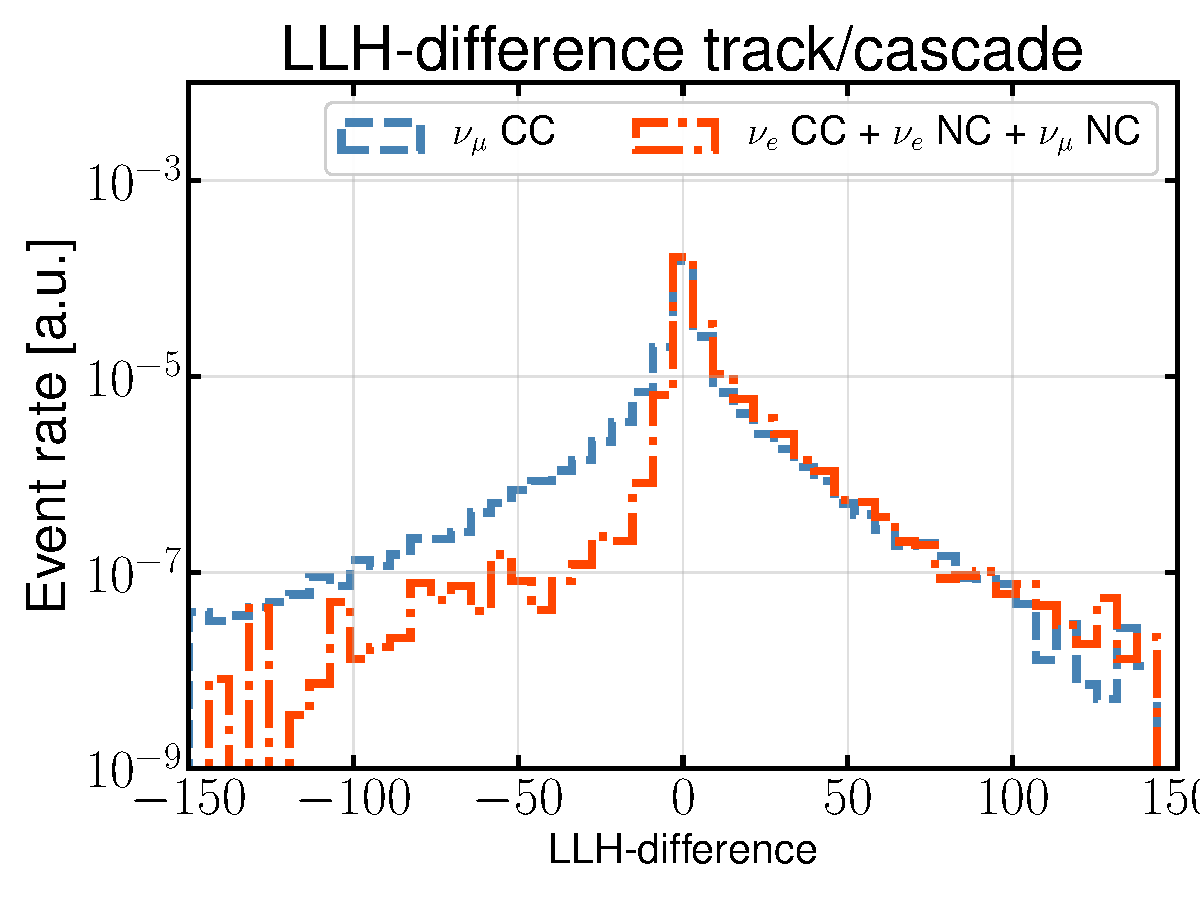
\includegraphics[width=0.49\linewidth]{figures/icecube/classification/variables/leera.pdf}
    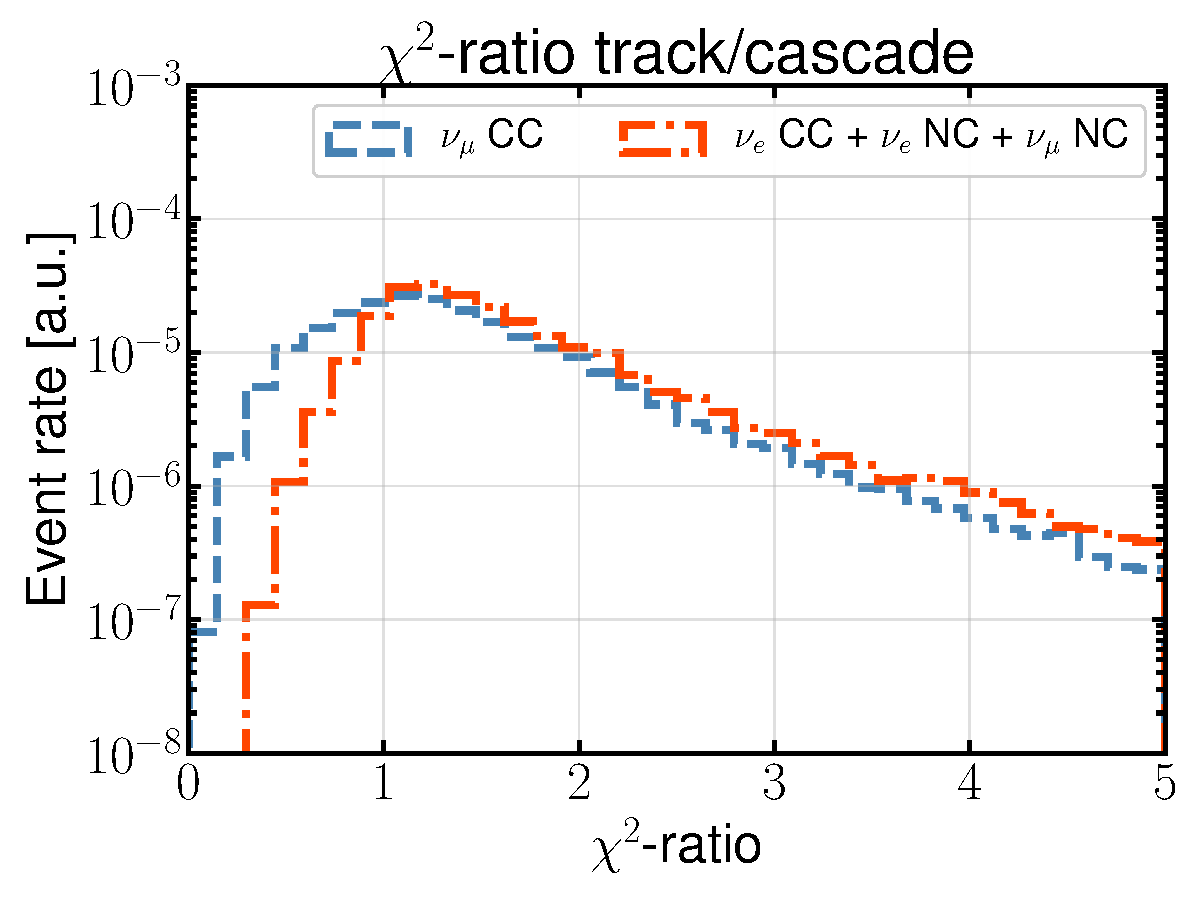
\includegraphics[width=0.49\linewidth]{figures/icecube/classification/variables/santa.pdf}
    \caption{Histograms of the likelihood score from the energy reconstruction (left) and the goodness-of-fit ratio of the zenith reconstruction (right) in simulation.}
    \label{fig:apx-pidvars-santa-leera}
\end{figure*}

\begin{figure*}
    \centering
    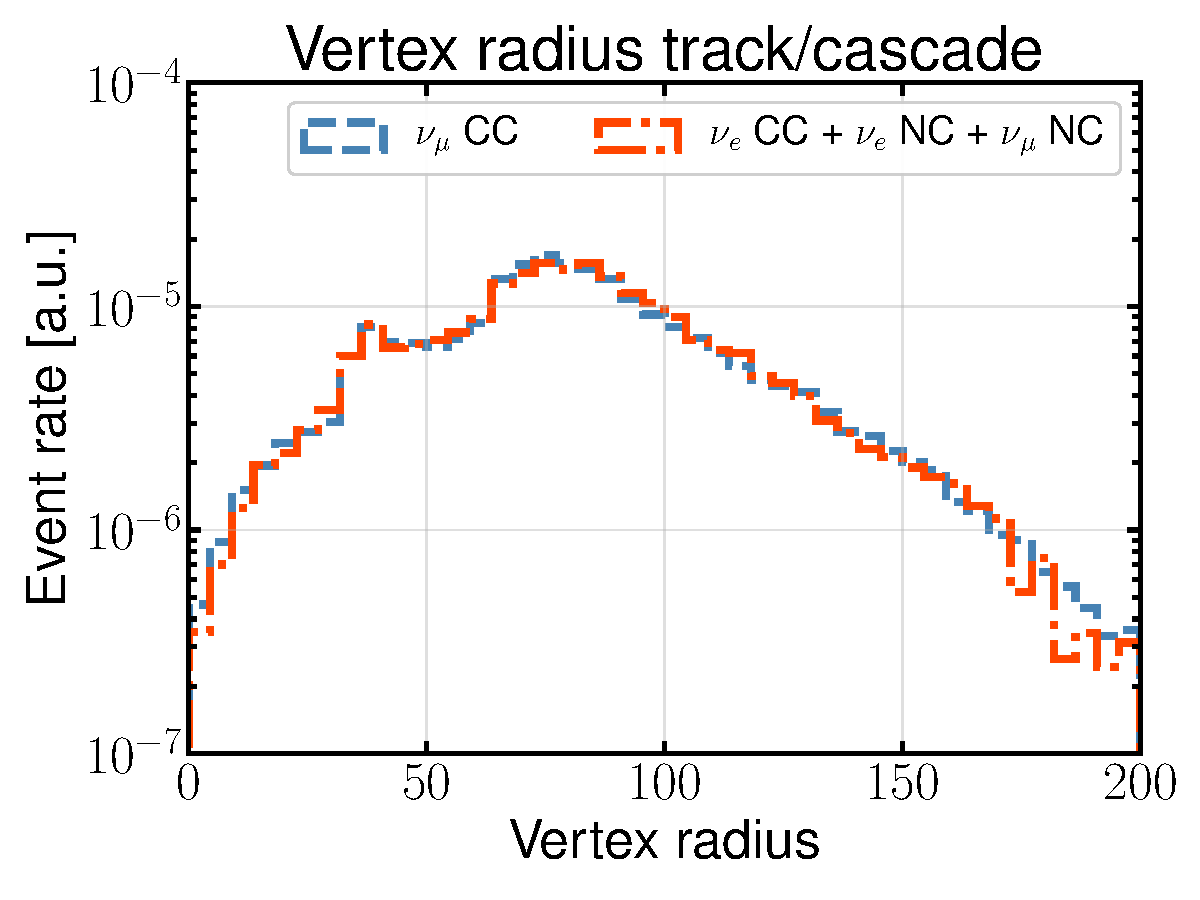
\includegraphics[width=0.49\linewidth]{figures/icecube/classification/variables/rho36_start.pdf}
    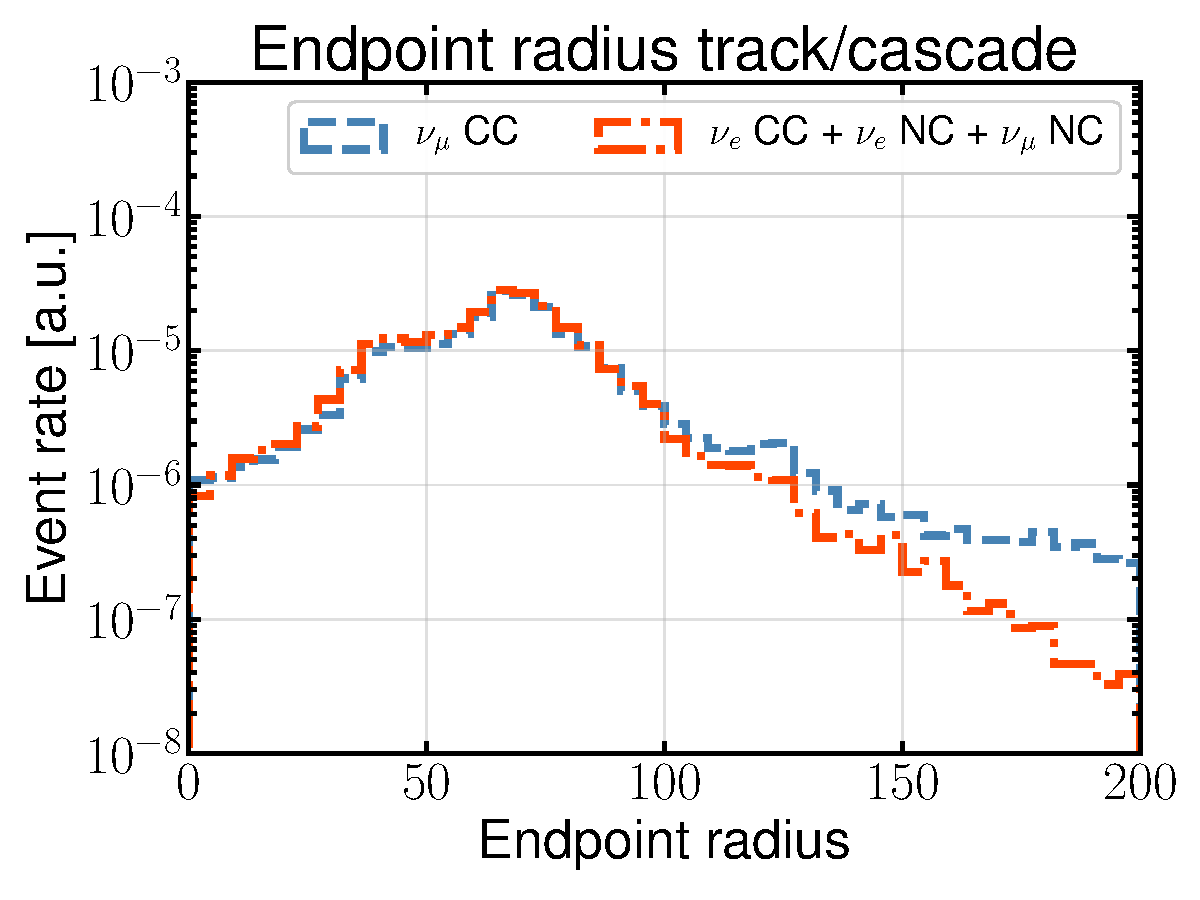
\includegraphics[width=0.49\linewidth]{figures/icecube/classification/variables/rho36_end.pdf}
    \caption{Histograms of the radius with respect to string 36 of the vertex (left) and the endpoint of the reconstructed track (right) in simulation.}
    \label{fig:apx-pidvars-rho36}
\end{figure*}

\begin{figure*}
    \centering
    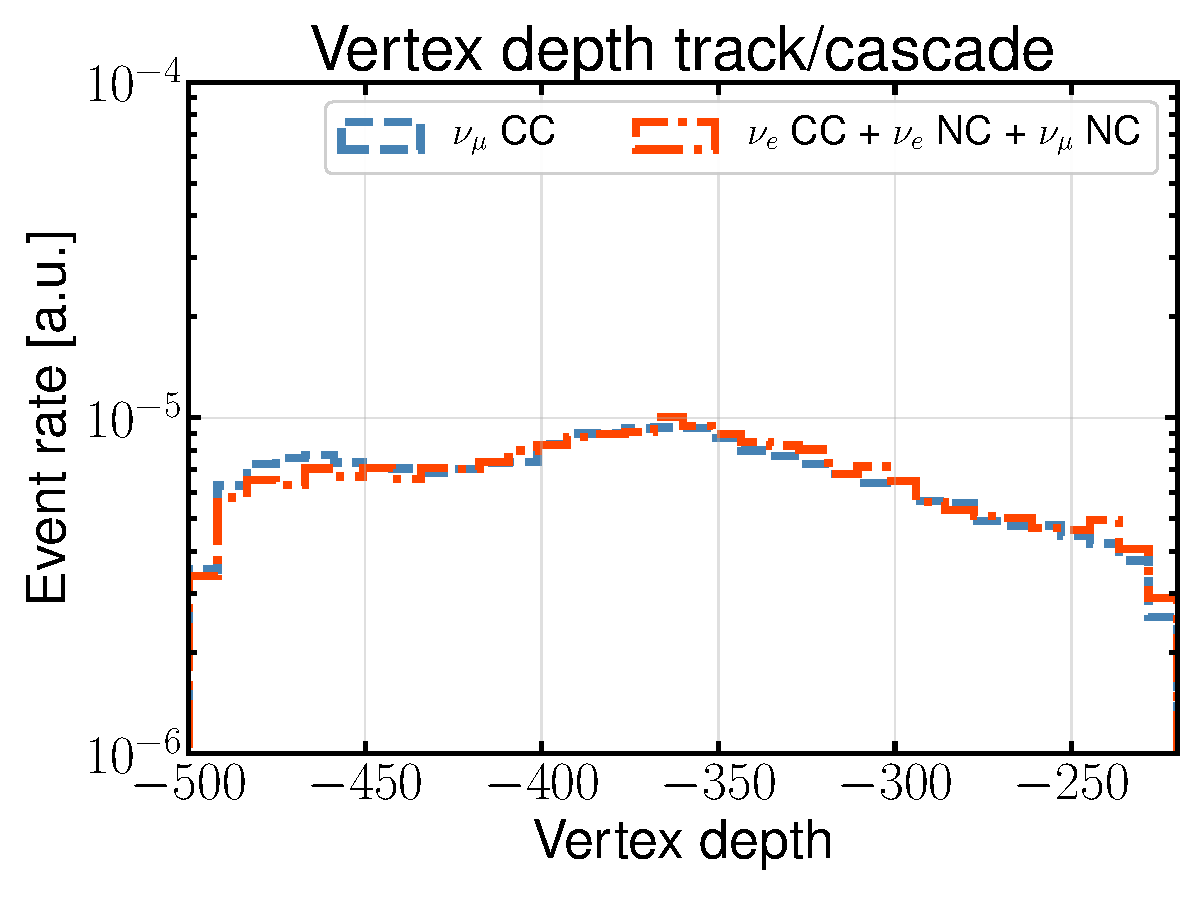
\includegraphics[width=0.49\linewidth]{figures/icecube/classification/variables/z_start.pdf}
    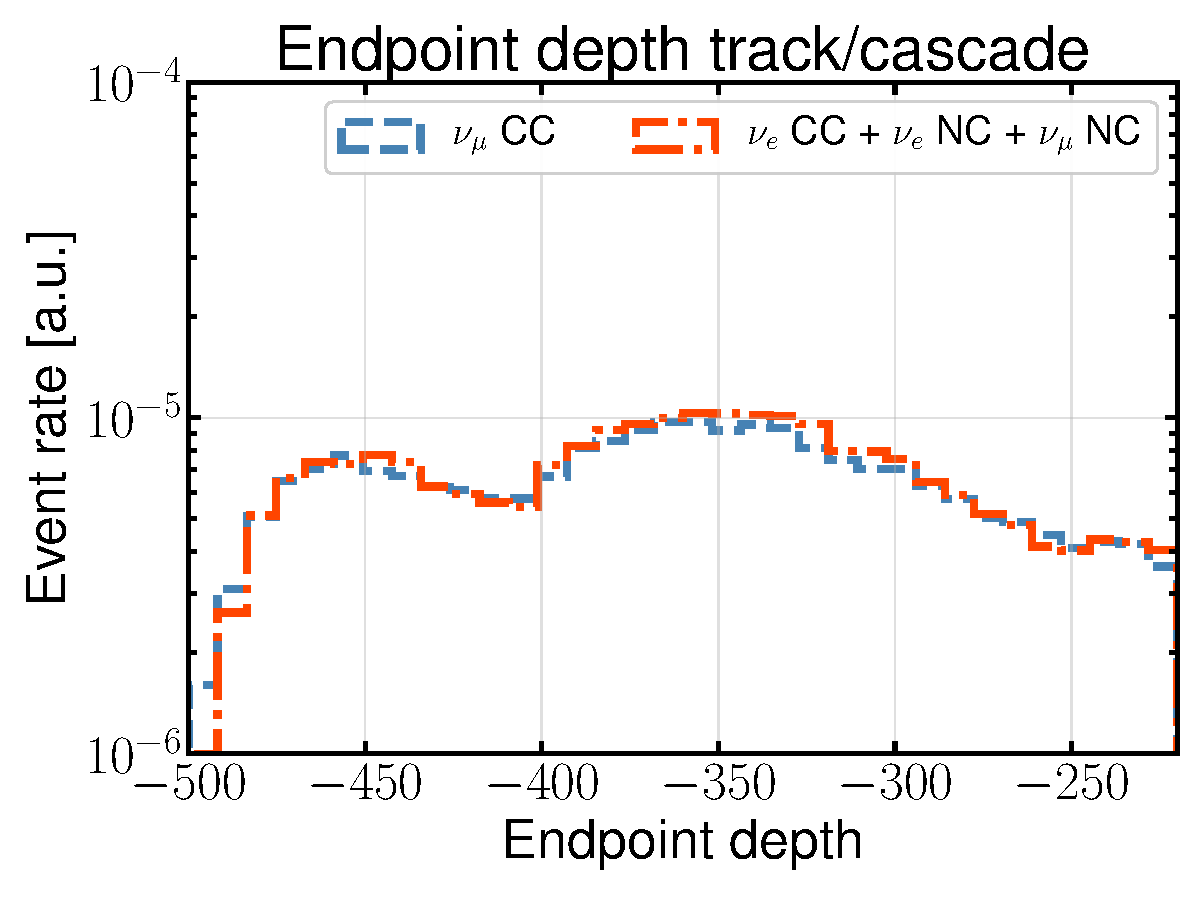
\includegraphics[width=0.49\linewidth]{figures/icecube/classification/variables/z_end.pdf}
    \caption{Histograms of the z-coordinate of the vertex (left) and the endpoint of the reconstructed track (right) in simulation.}
    \label{fig:apx-pidvars-z}
\end{figure*}

\begin{figure*}
    \centering
    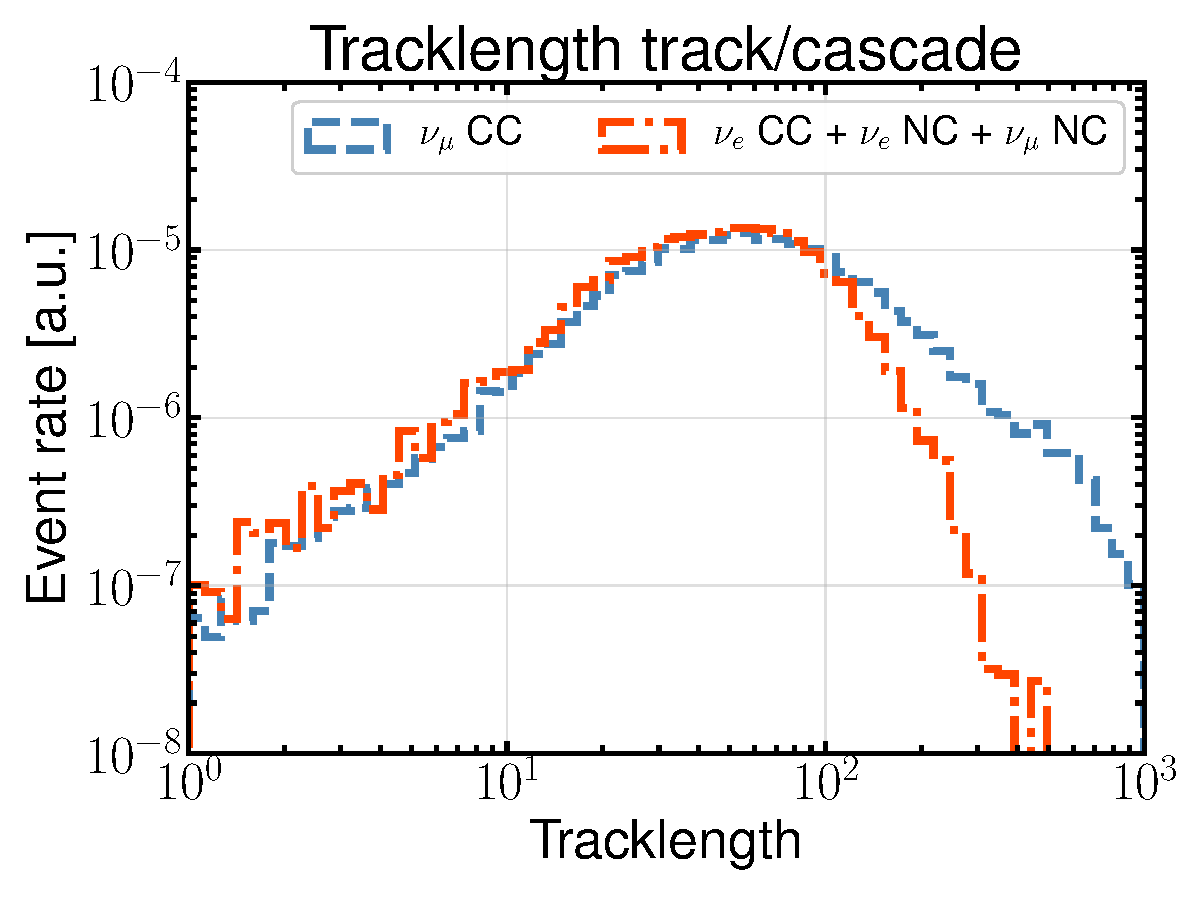
\includegraphics[width=0.49\linewidth]{figures/icecube/classification/variables/tracklength.pdf}
    \caption{Histogram of the reconstructed track length in simulation.}
    \label{fig:apx-pidvars-length}
\end{figure*}